\input{../YKY-preamble.tex}
\setmainfont[BoldFont=AlibabaSans-Regular.otf]{AlibabaSans-Light.otf}

\usepackage[active,tightpage]{preview}		% for continuous page(s)
\renewcommand{\PreviewBorder}{0.5cm}
\renewcommand{\thempfootnote}{\arabic{mpfootnote}}

\usepackage[absolute,overlay]{textpos}		% for page number on upper left corner

\usepackage{color}
\usepackage{mathtools}
\usepackage[hyperfootnotes=false]{hyperref}

% \usepackage[backend=biber,style=numeric]{biblatex}
% \bibliography{../AGI-book}
% \renewcommand*{\bibfont}{\footnotesize}

\usetikzlibrary{shapes}
\usepackage[export]{adjustbox}				% ??
\usepackage{bm}
\usepackage{verbatim} % for comments
% \usepackage[most]{tcolorbox}
% \usepackage{newtxtext,newtxmath}	% Times New Roman font

% \numberwithin{equation}{subsection}

\newcommand{\underdash}[1]{%
	\tikz[baseline=(toUnderline.base)]{
		\node[inner sep=1pt,outer sep=10pt] (toUnderline) {#1};
		\draw[dashed] ([yshift=-0pt]toUnderline.south west) -- ([yshift=-0pt]toUnderline.south east);
	}%
}%

%\DeclareSymbolFont{symbolsC}{U}{txsyc}{m}{n}
%\DeclareMathSymbol{\strictif}{\mathrel}{symbolsC}{74}
\DeclareSymbolFont{AMSb}{U}{msb}{m}{n}
\DeclareSymbolFontAlphabet{\mathbb}{AMSb}
% \setmathfont{Latin Modern Math}

% \newcommand{\highlight}[1]{\colorbox{pink}{$\displaystyle #1$}}

% \newcommand{\emp}[1]{{\color{violet}\textbf{#1}}}
\let\oldtextbf\textbf
\renewcommand{\textbf}[1]{\textcolor{blue}{\oldtextbf{#1}}}

\newcommand*\confoundFace{$\vcenter{\hbox{\includegraphics[scale=0.2]{../2020/../confounded-face.jpg}}}$}
\newcommand{\underconst}{\includegraphics[scale=0.5]{../2020/UnderConst.png}}
\newcommand{\KBsymbol}{\vcenter{\hbox{\includegraphics[scale=1]{../KB-symbol.png}}}}
\newcommand{\witness}{\scalebox{0.6}{$\blacksquare$}}
% \newcommand{\Heytingarrow}{\mathrel{-}\mathrel{\triangleright}}
% \providecommand\Heytingarrow{\relbar\joinrel\mathrel{\vcenter{\hbox{\scalebox{0.75}{$\rhd$}}}}}

\begin{document}

\begin{preview}

\cc{
\title{\vspace{-2.2cm} \bfseries\color{blue}{\large 大脑与 Transformer}}
}{
\title{\vspace{-2.2cm} \bfseries\color{blue}{\large Brain vs Transformer}}
}

% \author{YKY} % Your name
\date{\vspace{-3.2cm}} % Date, can be changed to a custom date

\maketitle

\setcounter{section}{0}

% (1) Circled page number on upper left corner
\begin{textblock*}{5cm}(2.1cm,2.3cm) % {block width} (coords) 
{\color{red}{\large \textcircled{\small 1}}}
\end{textblock*}

\begin{minipage}{\textwidth}
\setlength{\parskip}{0.4\baselineskip}

\vspace*{0.3cm} 

There are two distinct aspects in the brain:
	\begin{itemize}
		\item \textbf{Short-term} or Working Memory is the \textbf{electric activation} of neuronal populations.
		\item \textbf{Long-term} memory is stored as \textbf{synaptic strengths}, established by synaptic formation and strengthening.  The transfer from STM to LTM is called \textbf{memory consolidation}.
	\end{itemize}
	
One theory has it that the prefrontal cortex maintains a number of ``thoughts'' with sub-populations or, perhaps, with \textbf{micro-columns}.  These activated sub-populations are in competition with each other, through \textbf{lateral inhibition}.  The thought(s) that win are the thoughts we retain -- they ``make sense''.
	
\subsection{How does symbolic logic emerge in the brain?}

\subsubsection{Disentangled features}
	
If a room of people see a cat enter the room, one person will say ``There's a cat in the room!'' but afterwards it would be \textbf{redundant} for others to say exactly the same thing.  Likewise, in a neural network, if two output features both identify ``cat'' then they are redundant, a waste of resources.  So it is more efficient for one feature vector to move away to a new location in \textbf{feature space}:
	\begin{equation}
	\vcenter{\hbox{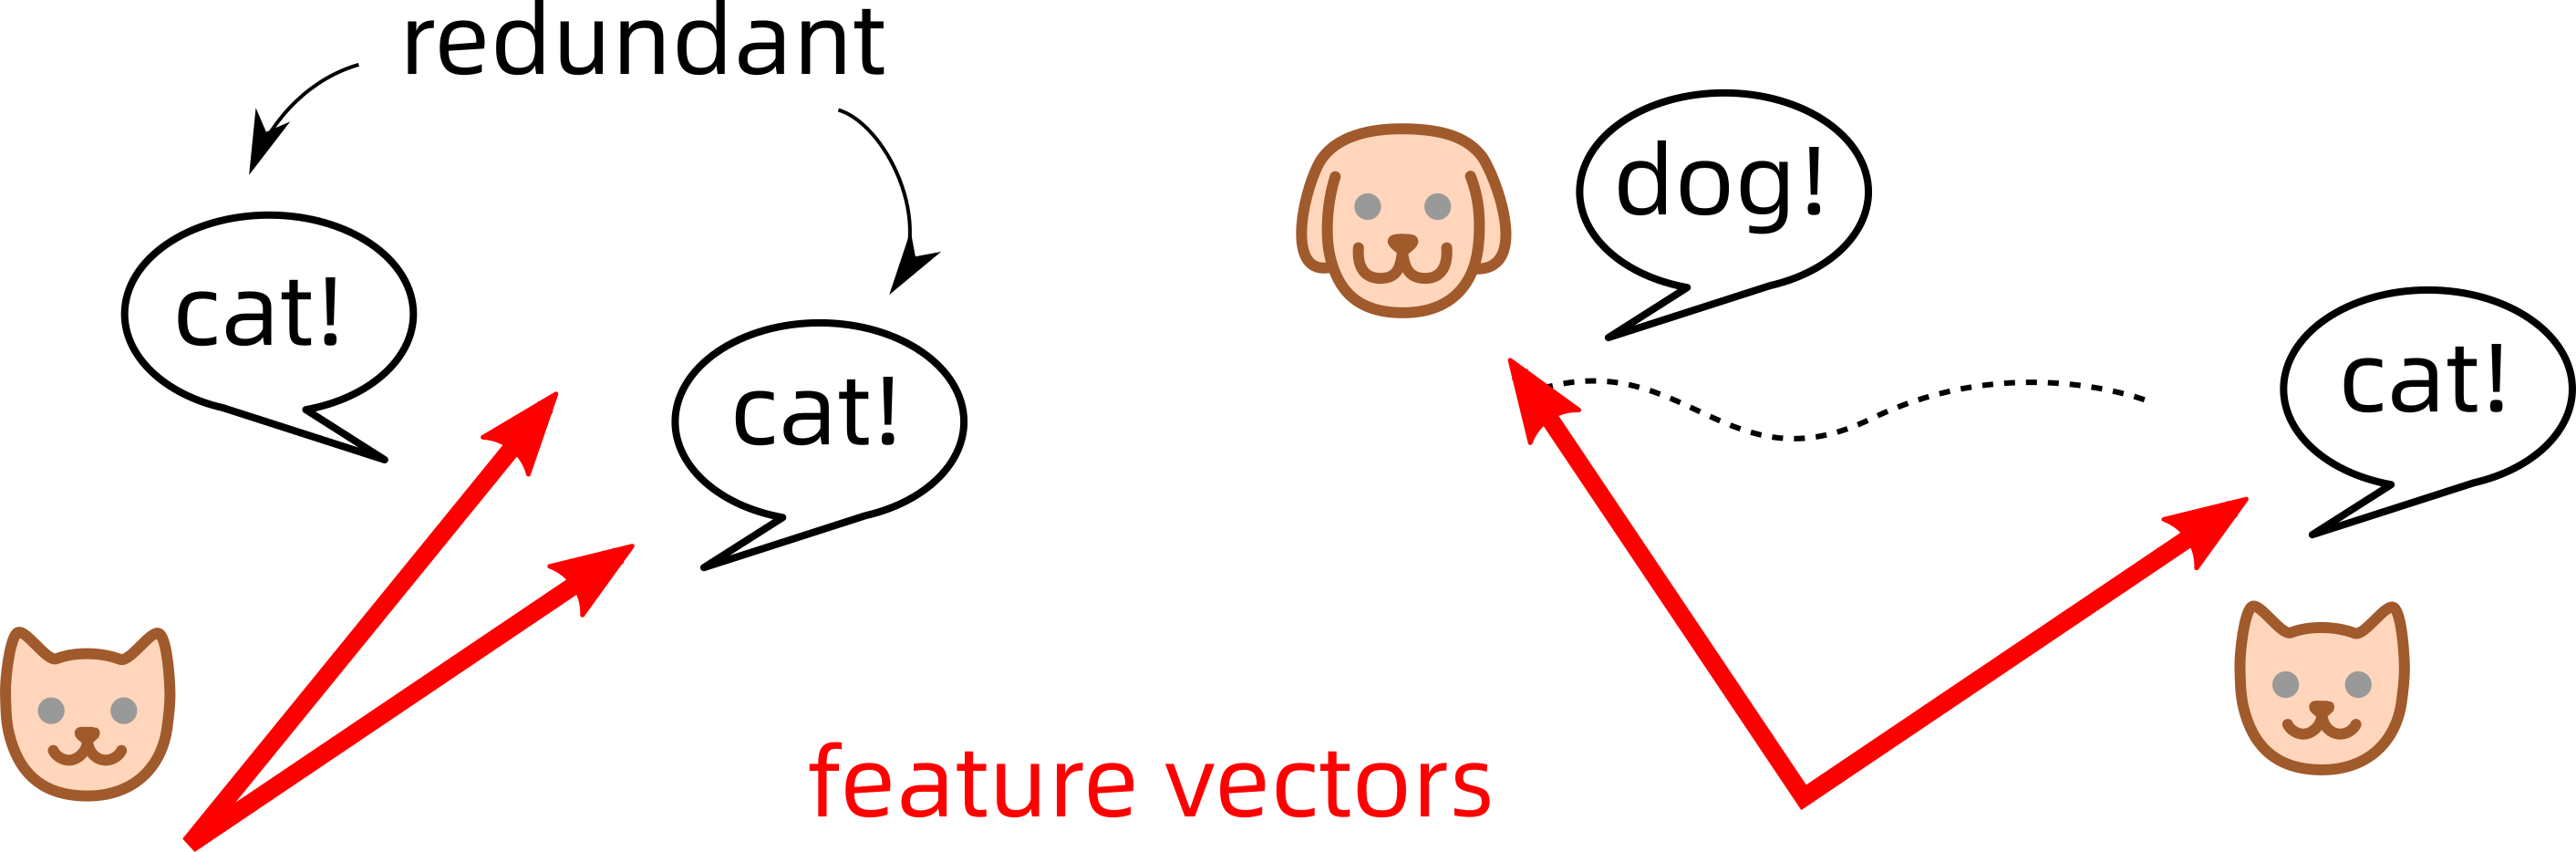
\includegraphics[scale=0.7]{disentangled-features.png}}}
	\end{equation}
	The result is the emergence of \textbf{disentangled features}.  There is now a lot of research papers on this topic;  Personally I first learned of this from Marta Garnelo and Murray Shanahan's paper  Shanahan2019.  We can think of this as a first step of \textbf{symbolization}, in which objects are recognized by symbols.
	
	In the cortex, neuronal populations are organized into ``columns'', with \textbf{lateral inhibition}  among themselves.  When one population is activated, it suppresses the activation of nearby populations.  This is likely to be the mechanism that enables disentangled features to emerge:
	\begin{equation}
	\vcenter{\hbox{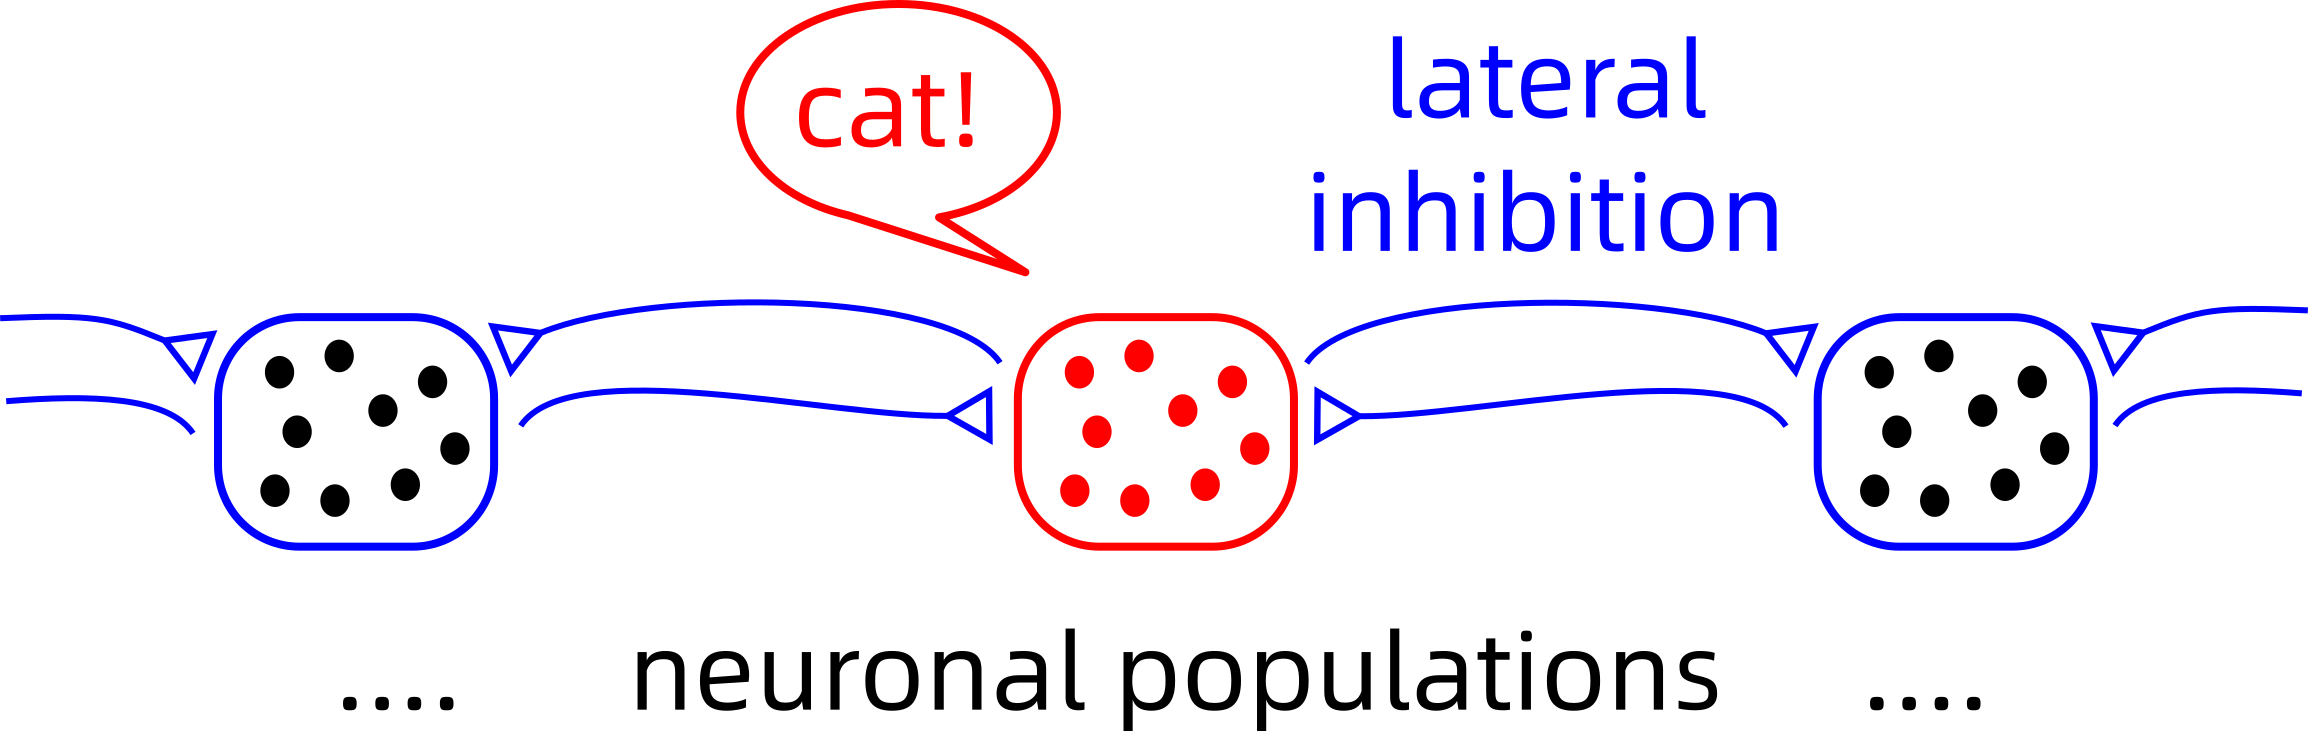
\includegraphics[scale=0.7]{lateral-inhibition.png}}}
	\end{equation}
	It is remarkable that the \textbf{softmax} in the Transformer / Self-Attention seems to be an abstract implementation of this winner-takes-all \textbf{selection} mechanism.
	
\subsubsection{Bi-directional connections in the cortex}
	
	Moreover, the cortex is organized into \textbf{layers} with widespread recurrent (ie, forward and backward) connections \footnote{More accurately, there exist two distinct structures: the cortex has a 6-layer structure which has recurrent connections within it;  and each cortical area has bi-directional connections to and from other areas (which may have hierarchical relations among themselves).  I have sort of glossed over this level of details.}:
	\begin{equation}
	\vcenter{\hbox{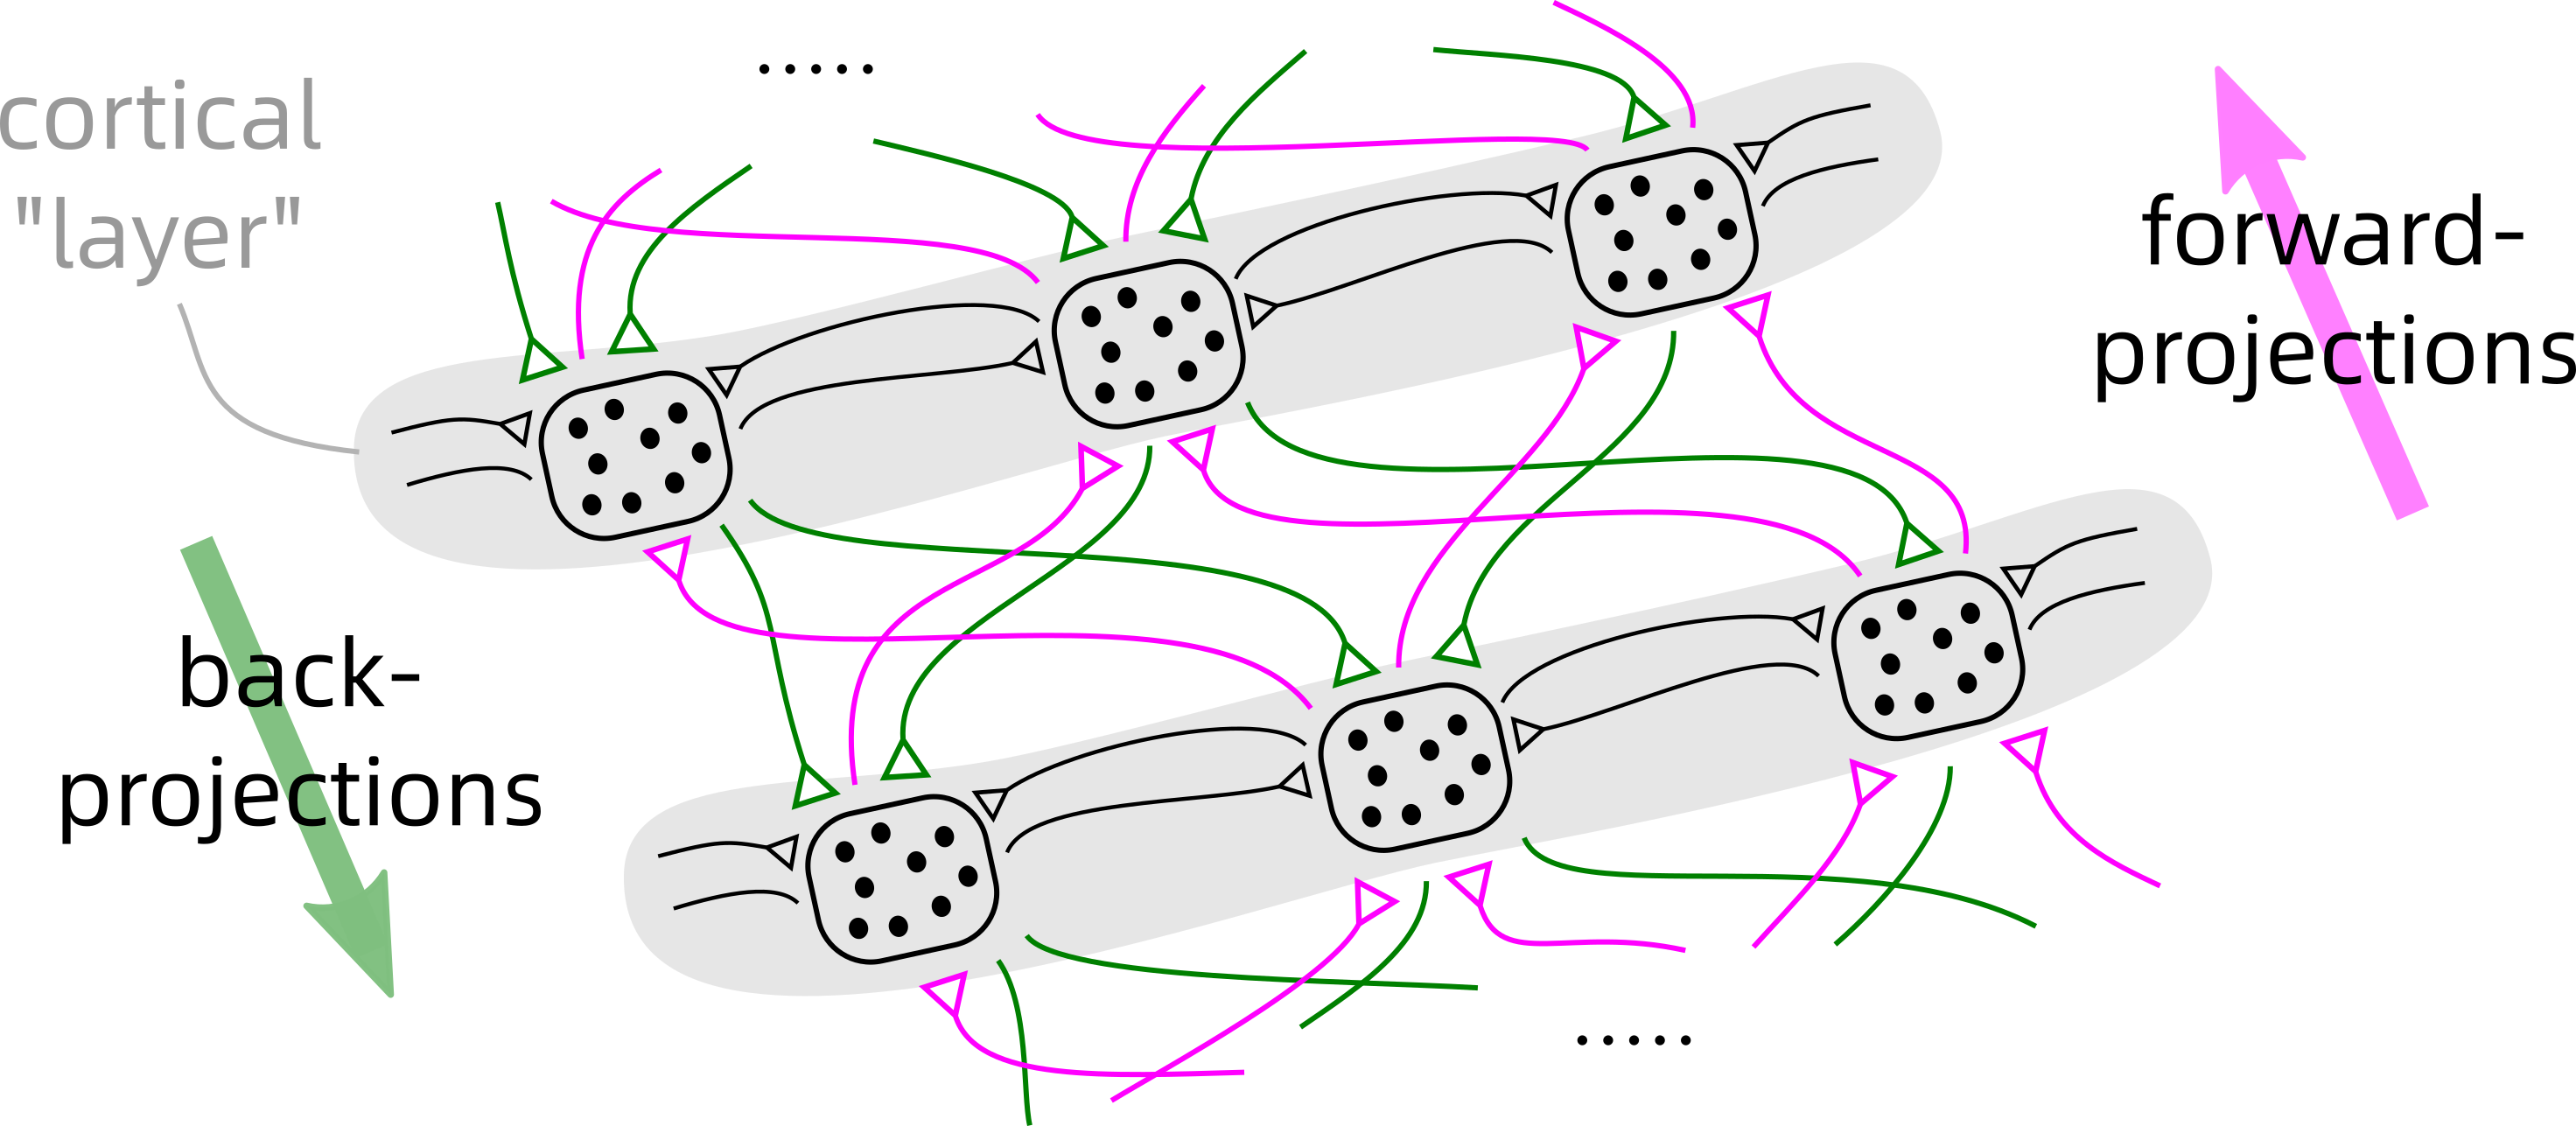
\includegraphics[scale=0.7]{cortex-back-projections.png}}}
	\label{fig:cortex-back-projections}
	\end{equation}
	This bi-directional architecture may be applicable to AGI architecture (see also \S\ref{sec:abductive-reasoning} on abductive reasoning), possibly replacing the current uni-directional model of feed-forward networks and the back-propagation algorithm.
	
\subsubsection{Alternative to back-propagation?}
	
As is well-known, the brain does not use back-prop.  The bi-directional innervation is a very significant brain architectural feature that has not yet been incorporated into current deep learning techniques.
	
In order to find an alternative to back-prop, we need to ask:  What is the essence of deep learning?  I think the answer lies in two words, ``hierarchical'' and ``learned''.  As a counter example, decision trees are hierarchical structures that are learned, but the learning algorithm is too slow because it uses combinatorial search (reminiscent of NP hardness).
	
But the brain must have a roughly equally powerful learning mechanism as back-prop.  A likely candidate is \textbf{resonance}.  In figure (\ref{fig:cortex-back-projections}) we have a hierarchically connected cortical structure.  What we need is some sort of ``infinitesimal'' learning rule.
	
\subsubsection{Hierarchy of features}
	
If we consider relations between objects, for example, ``spoon inside a glass'', this too can emerge out of disentanglement of features, because it is a very \textbf{economical} / efficient representation of a complex scene:
	\begin{equation}
	\vcenter{\hbox{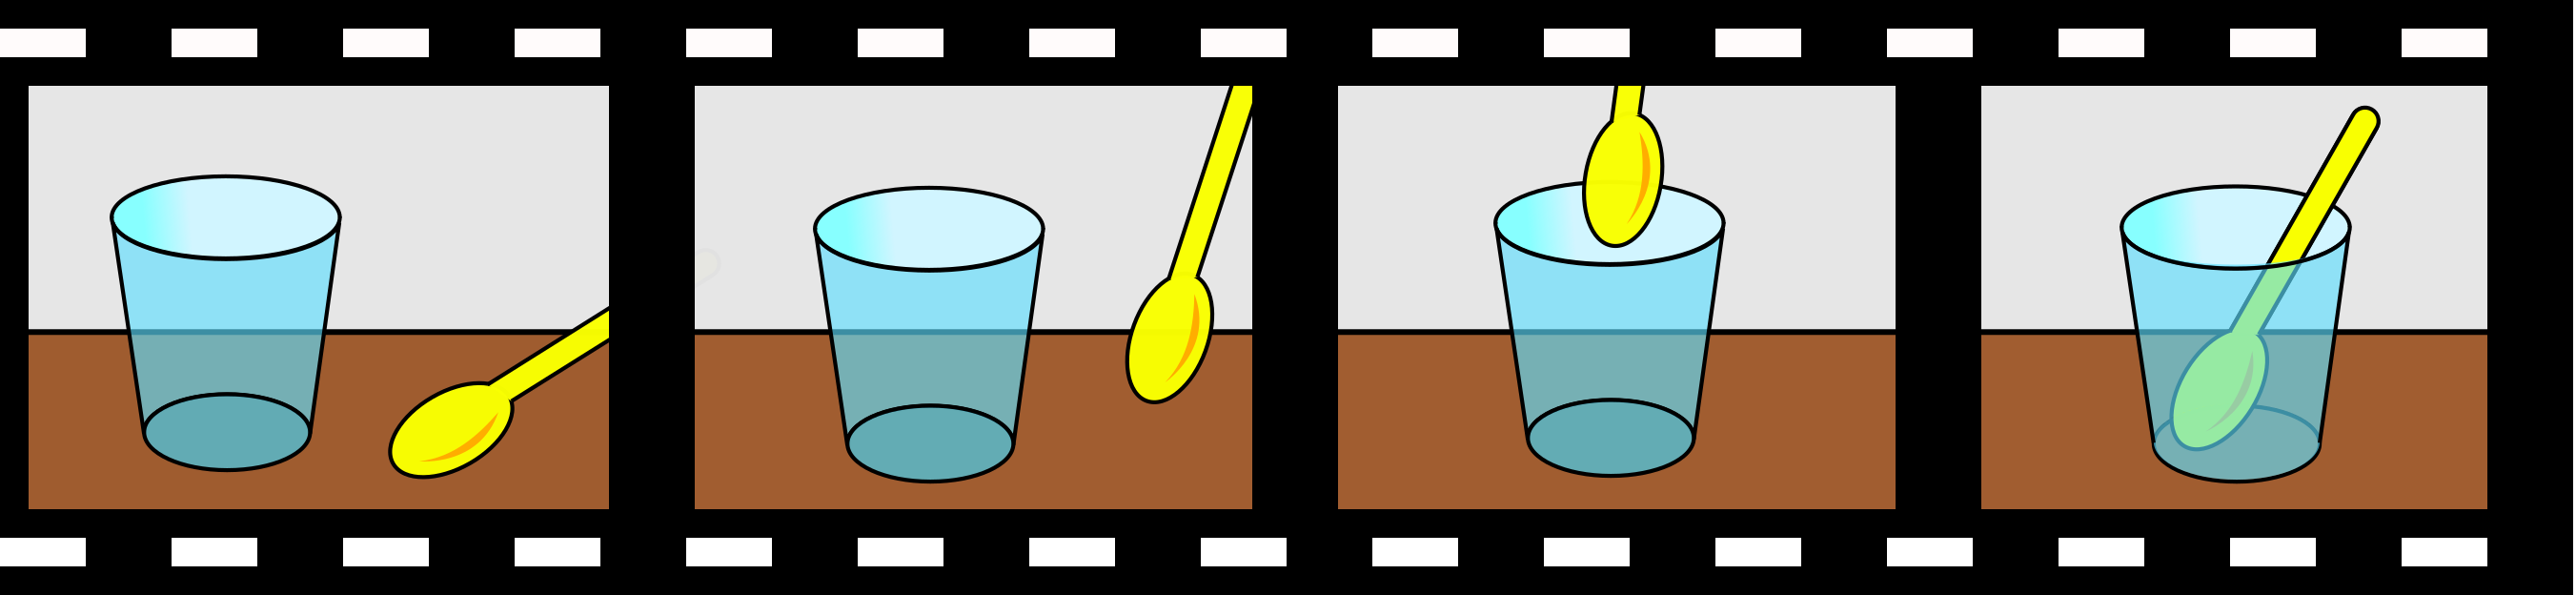
\includegraphics[scale=1]{spoon-in-glass-movie.png}}}
	\end{equation}
	Every human can recognize this as ``putting a spoon into a glass'', a symbolic representation.  Many researchers may have under-estimated how much the brain uses symbolic reasoning, and my proposal is that AGI can be based entirely on it.  
	
	One remaining question is how to represent symbolic data in a ``neural'' manner.  A general form of symbolic data may be as a \textbf{tree}.  Taking inspiration from the cortex (\ref{fig:cortex-back-projections}), we may perhaps represent the tree / symbolic data as hierarchically organized neural \textbf{feature vectors}:
	\begin{equation}
	\vcenter{\hbox{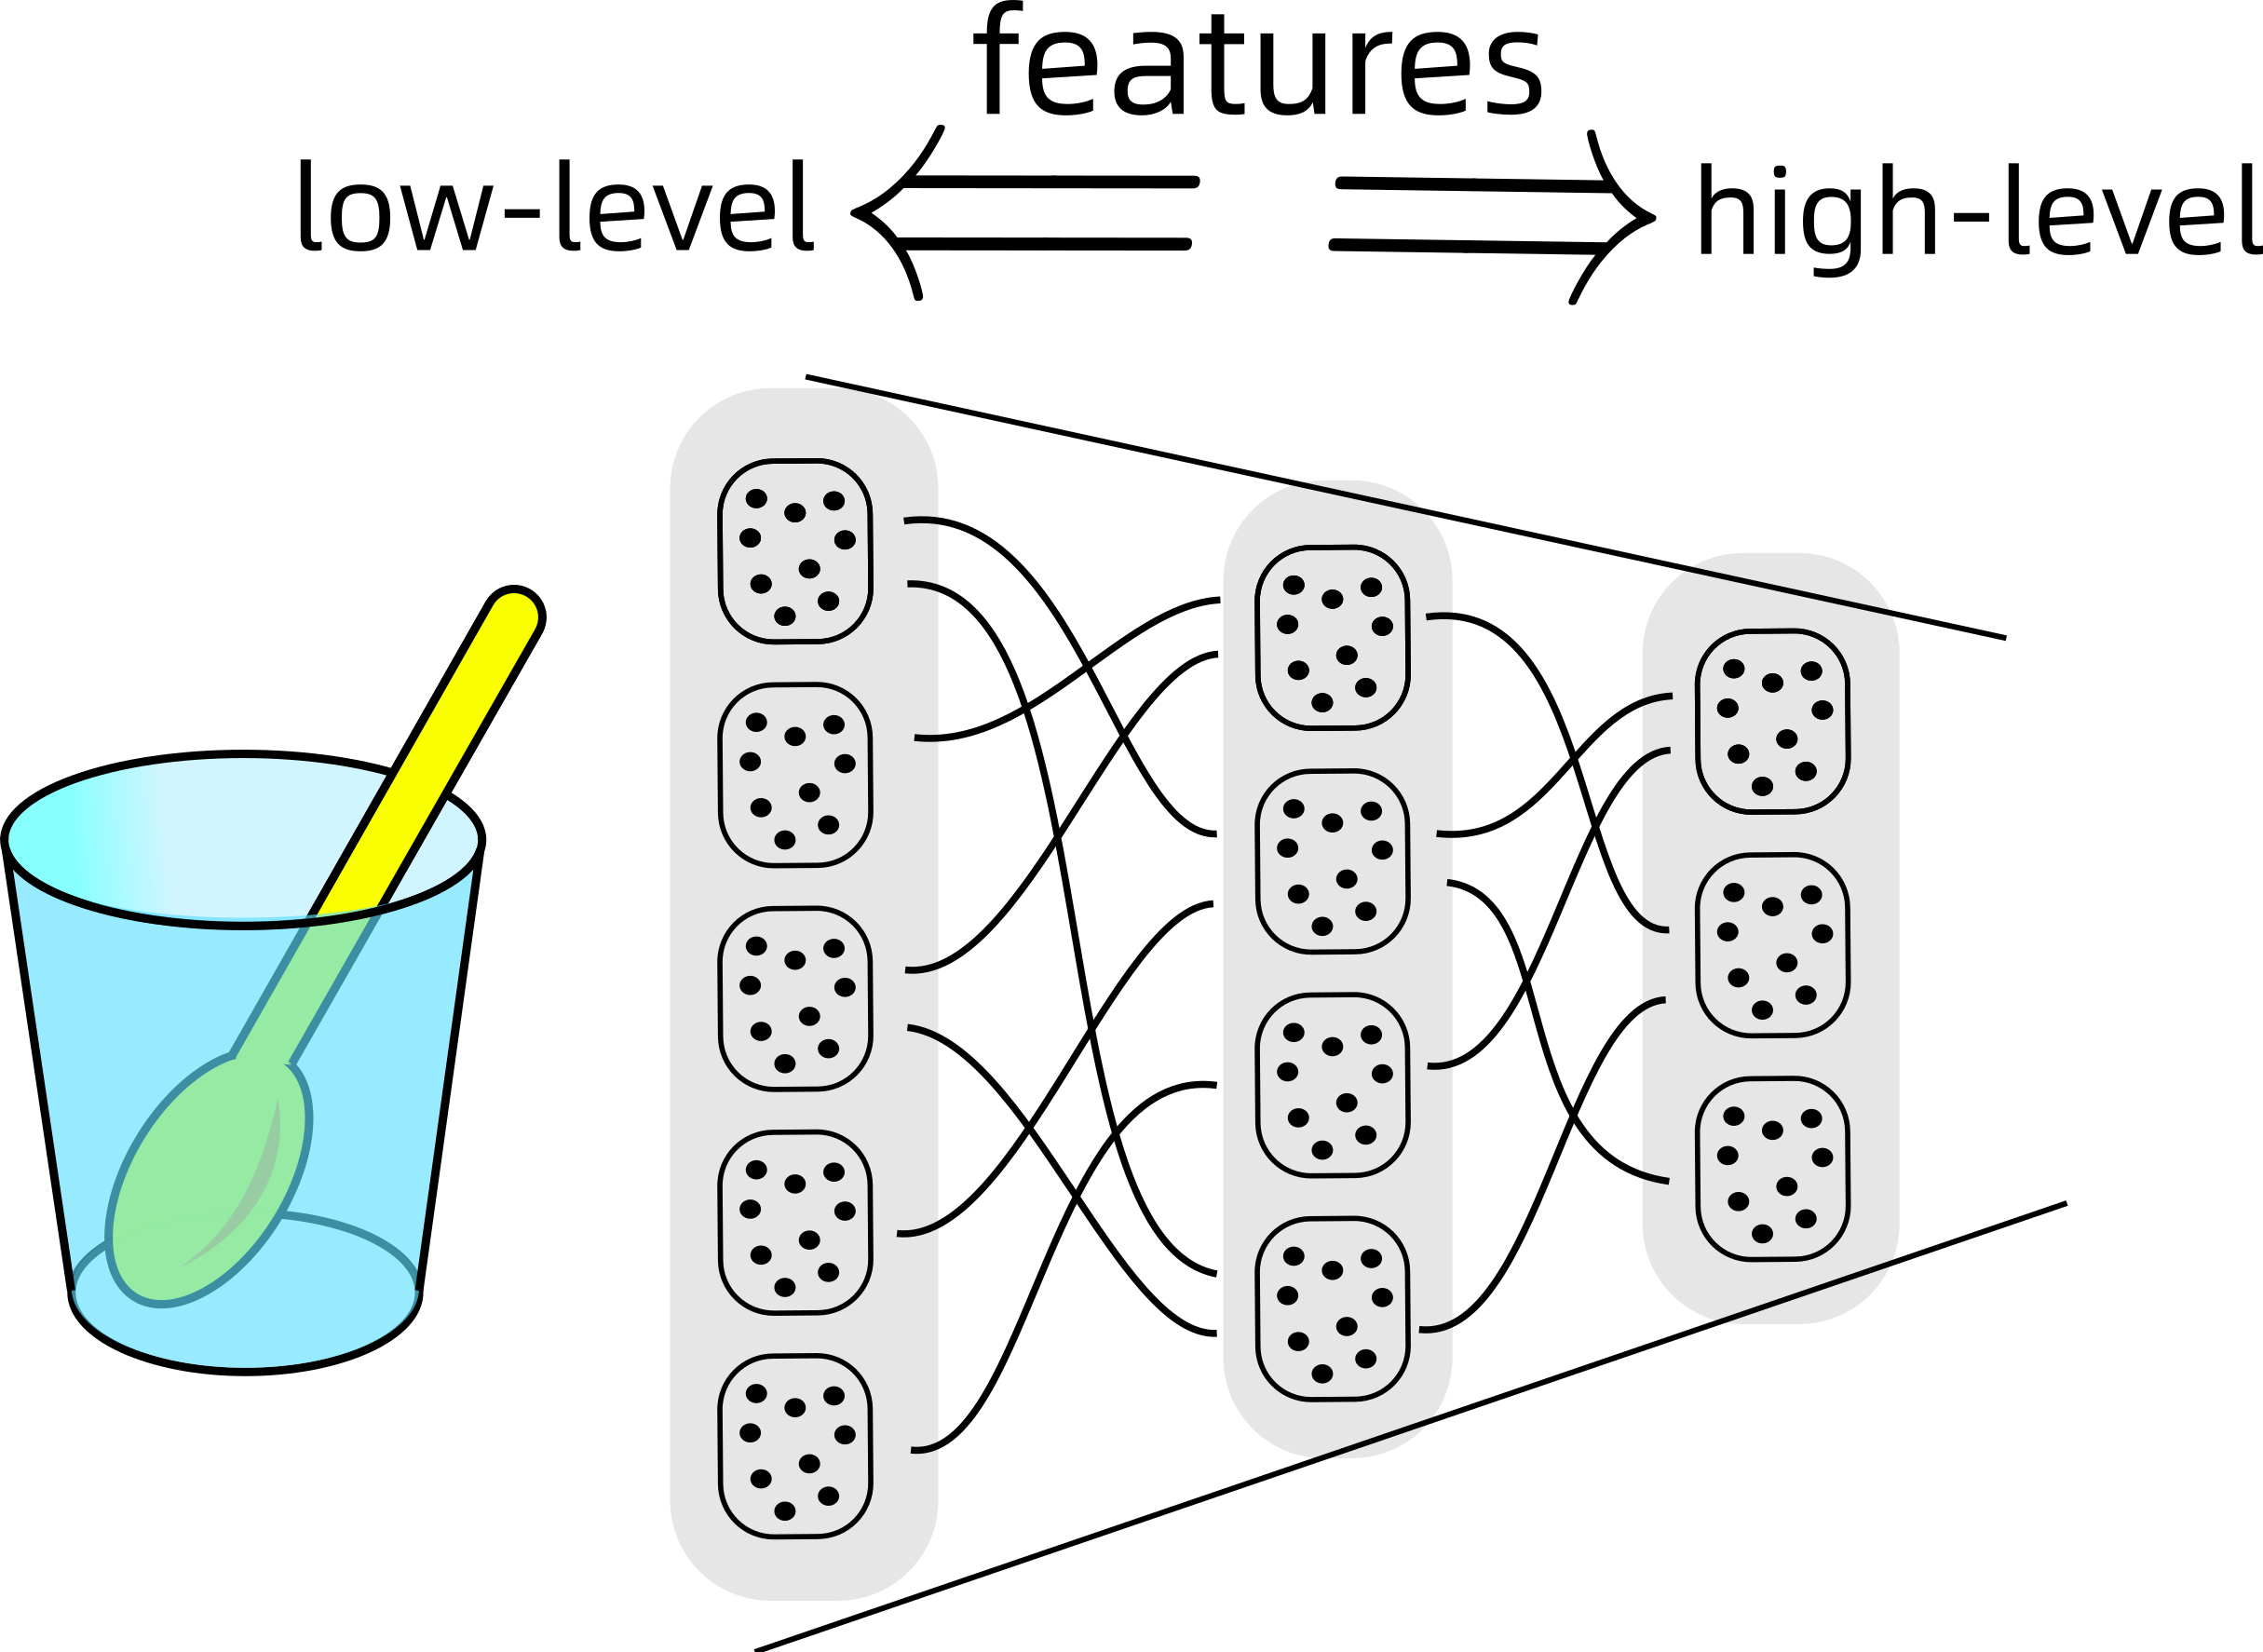
\includegraphics[scale=0.7]{hierarchical-features.png}}}
	\end{equation}
	
	Remember that in the Transformer, symbols are organized as \textbf{sequences}, for example: ``spoon $\cdot$ inside $\cdot$ glass.''  It may be desirable for AGI to have multiple levels of features, such as ``spoon'' and ``glass'' on a lower level, and ``inside'' on a higher level.
	
	Juxtaposed side by side, the Transformer and the cortex seem to have many similarities:
	\begin{equation}
	\vcenter{\hbox{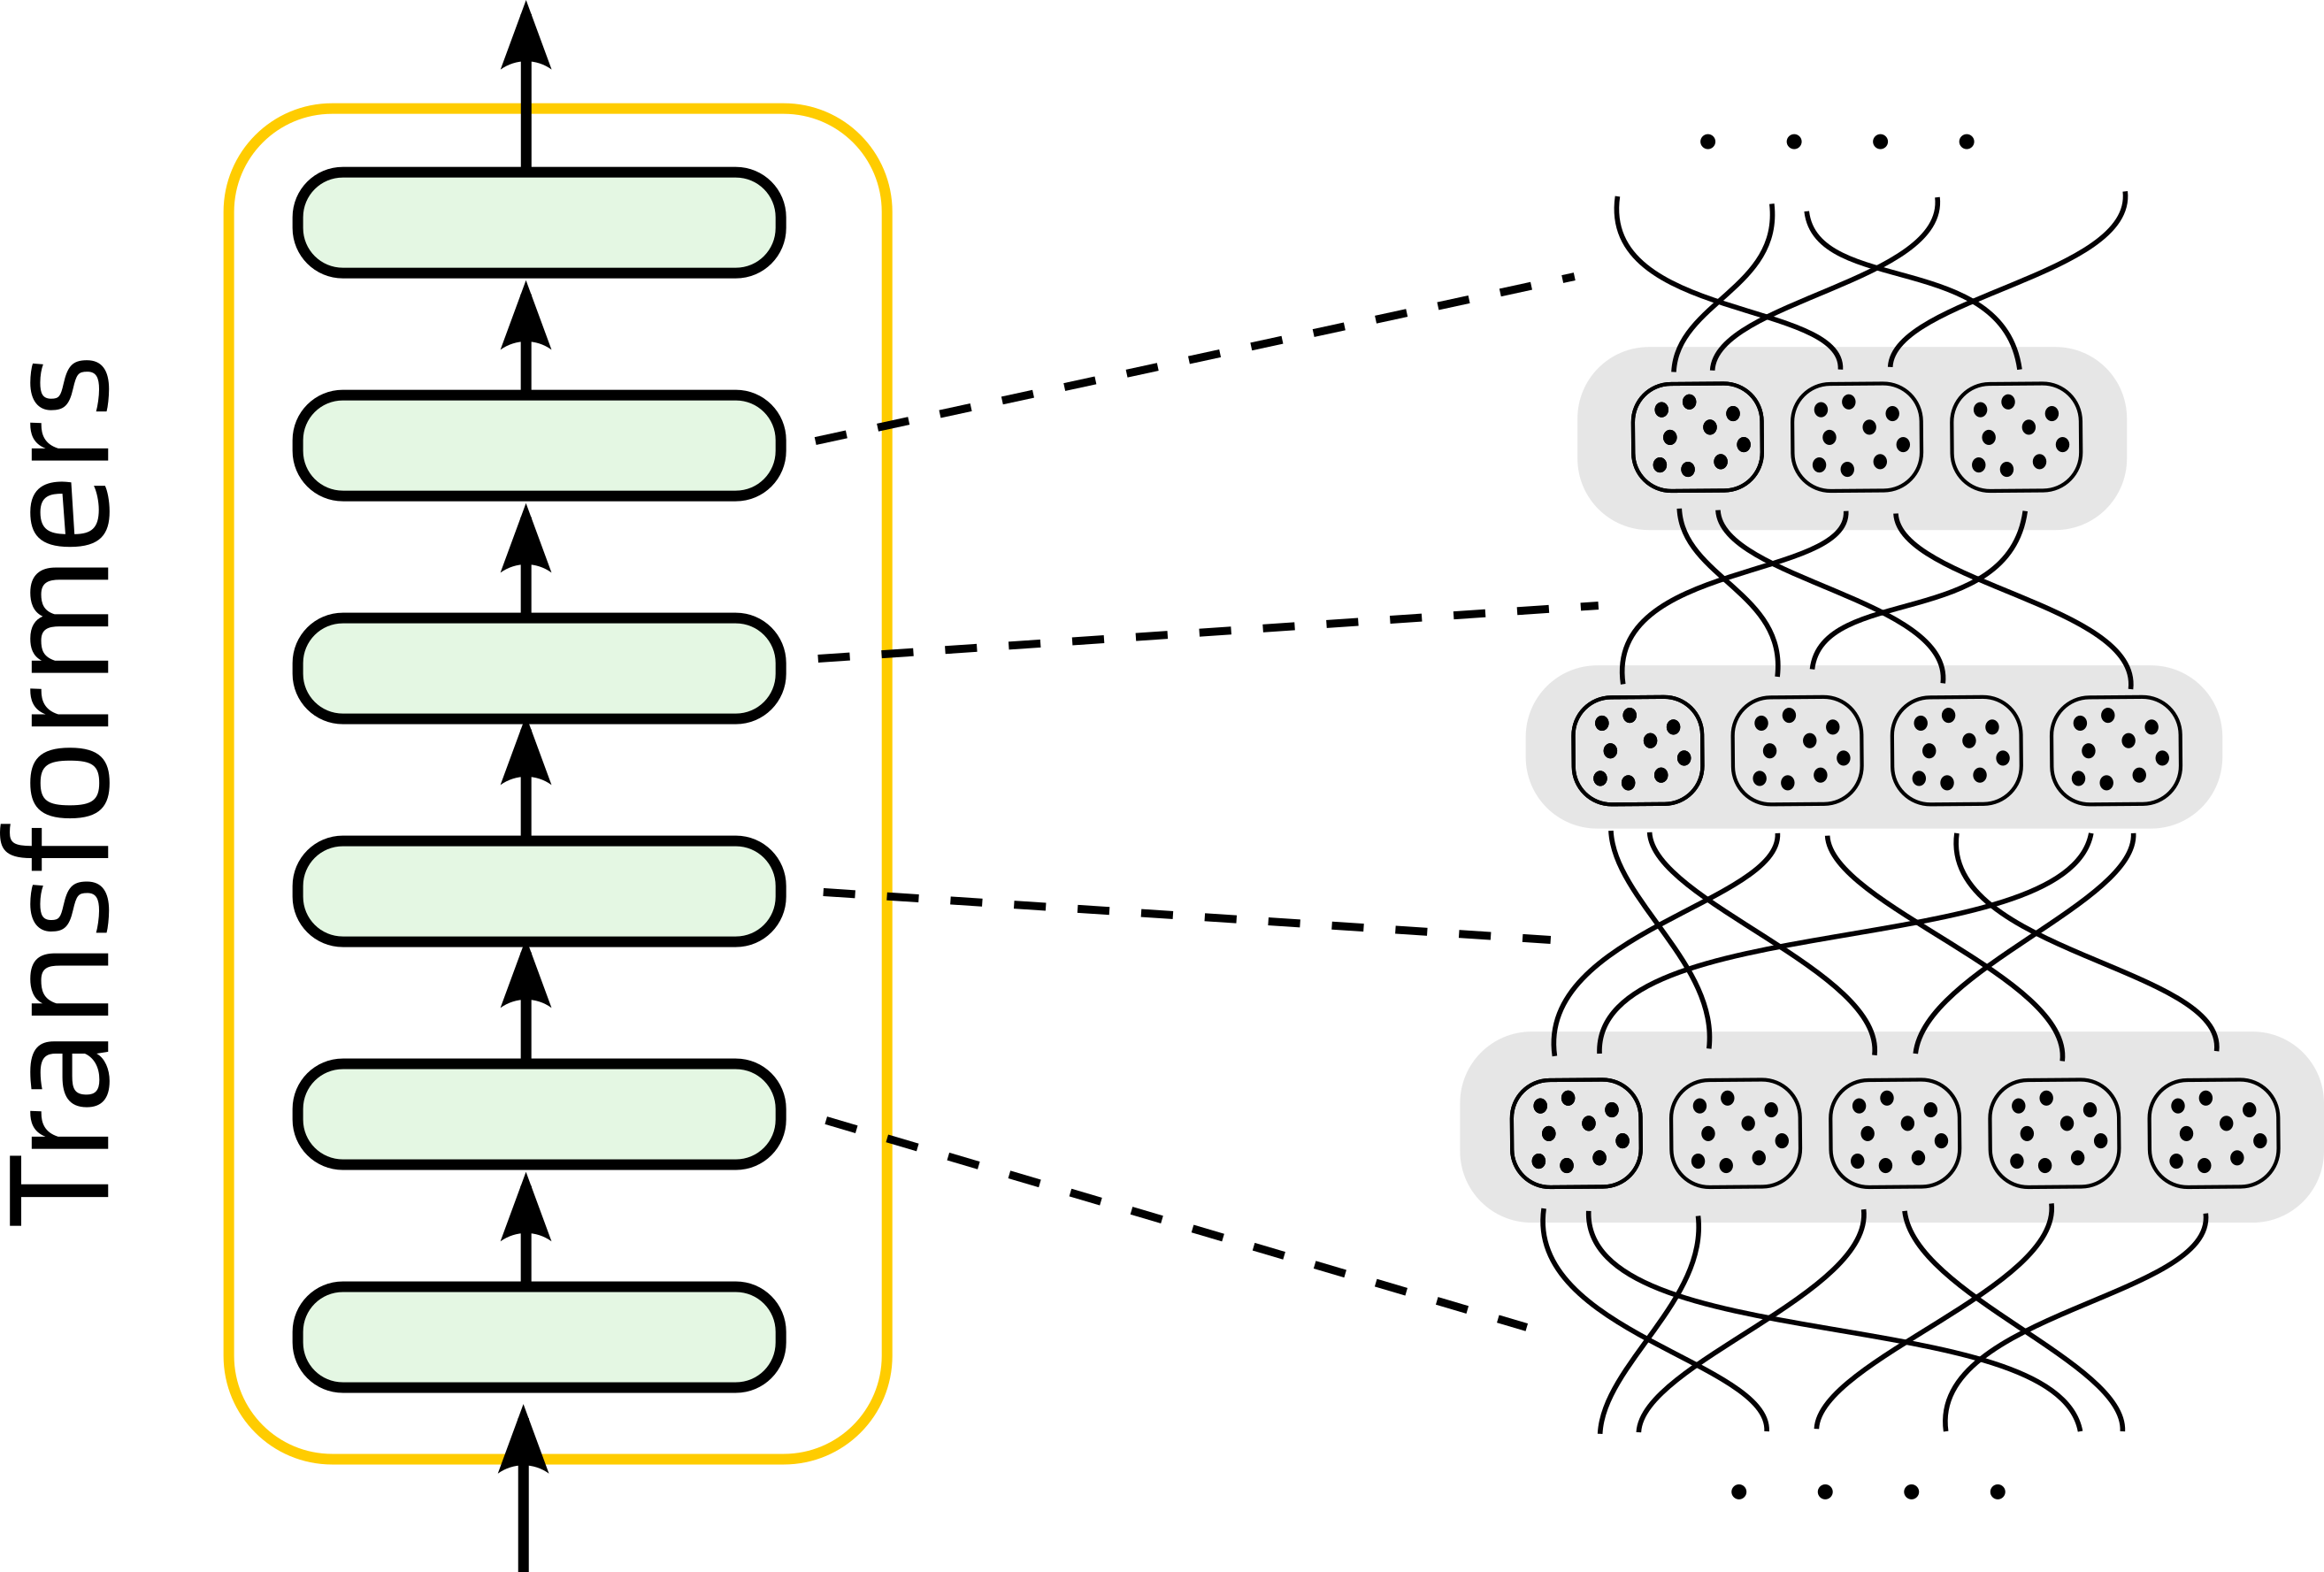
\includegraphics[scale=0.7]{Transformer-cortex-correspondence.png}}}
	\end{equation}
	Softmax corresponds to lateral inhibition.  The Transformer has many layers because it \textbf{unfolds} along the time axis the training of a recurrent network --- part of the reason why the Transformer is very efficient.  Each hidden layer of the Transformer can be construed as a ``stage'' of logical inference:
	\begin{equation}
	\mbox{input} \vdash \mbox{stage}_1 \vdash \mbox{stage}_2 \vdash .... \vdash \mbox{output}.
	\end{equation}
	
	Also recall that our reinforcement learning model consists of just the state and its transition function:
	\begin{equation}
	\vcenter{\hbox{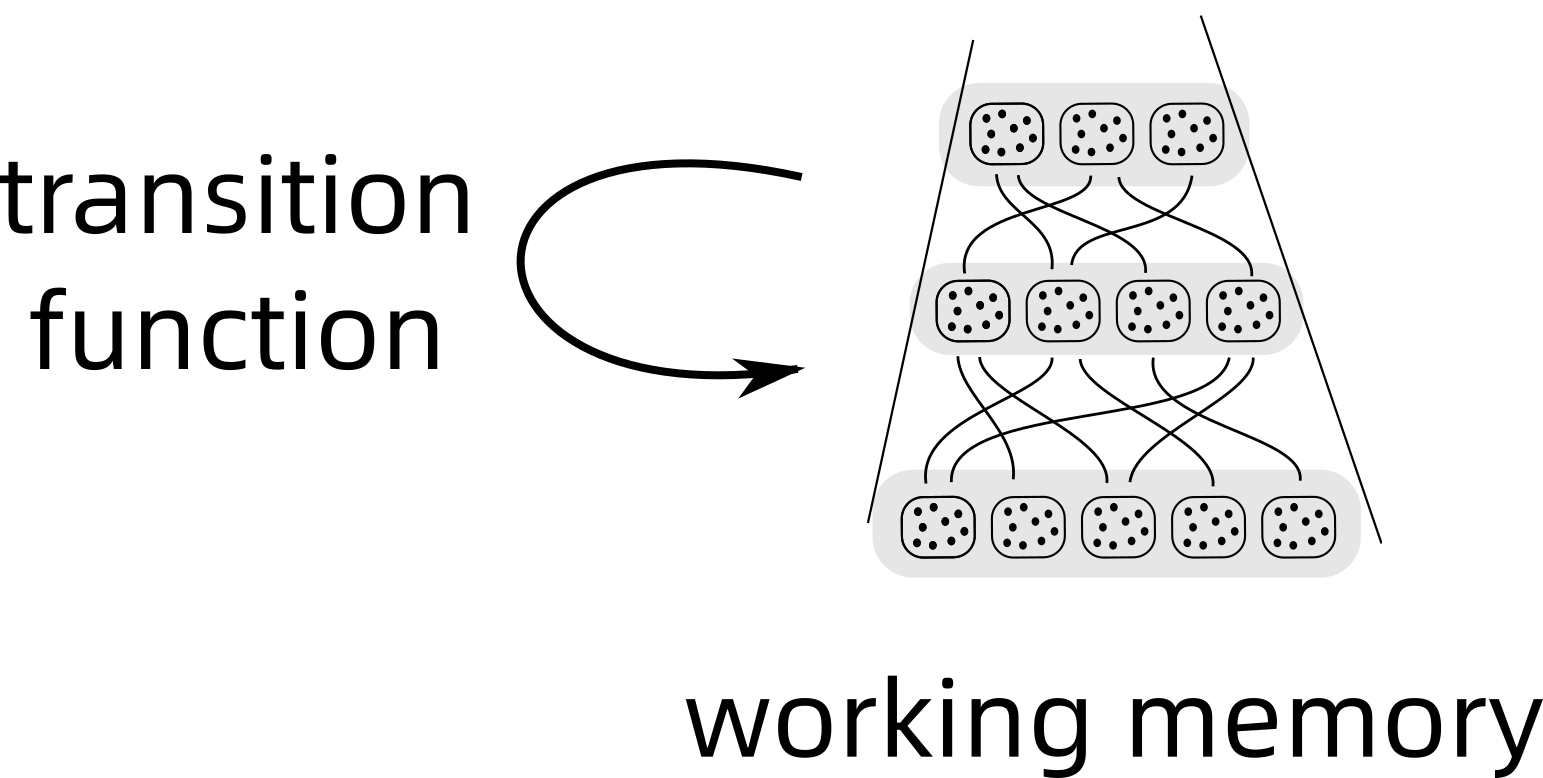
\includegraphics[scale=0.7]{cortex-with-transition-function.png}}}
	\end{equation}
	Based on this understanding, we need to figure out how to design the next version of Transformer and incorporate it into our AGI architecture....

\end{minipage}
\end{preview}
\end{document}